\documentclass[tikz,border=10pt]{standalone}
\usepackage{pgfplots}
\pgfplotsset{compat=newest}
% \pgfplotsset{compat=1.18}
\usepackage[american]{circuitikz}
\usepackage{cmbright}

\definecolor{myred}{RGB}{170,0,0}
\definecolor{myblue}{RGB}{0,0,220}
\definecolor{mygreen}{RGB}{0,150,0}
\definecolor{myorange}{RGB}{255,127,0}
\definecolor{mybrown}{RGB}{150,75,0}

\ctikzset{bipoles/resistor/height=0.2}
\ctikzset{bipoles/resistor/width=0.5}
\ctikzset{bipoles/capacitor/height=0.4}
\ctikzset{bipoles/capacitor/width=0.15}


\begin{document}

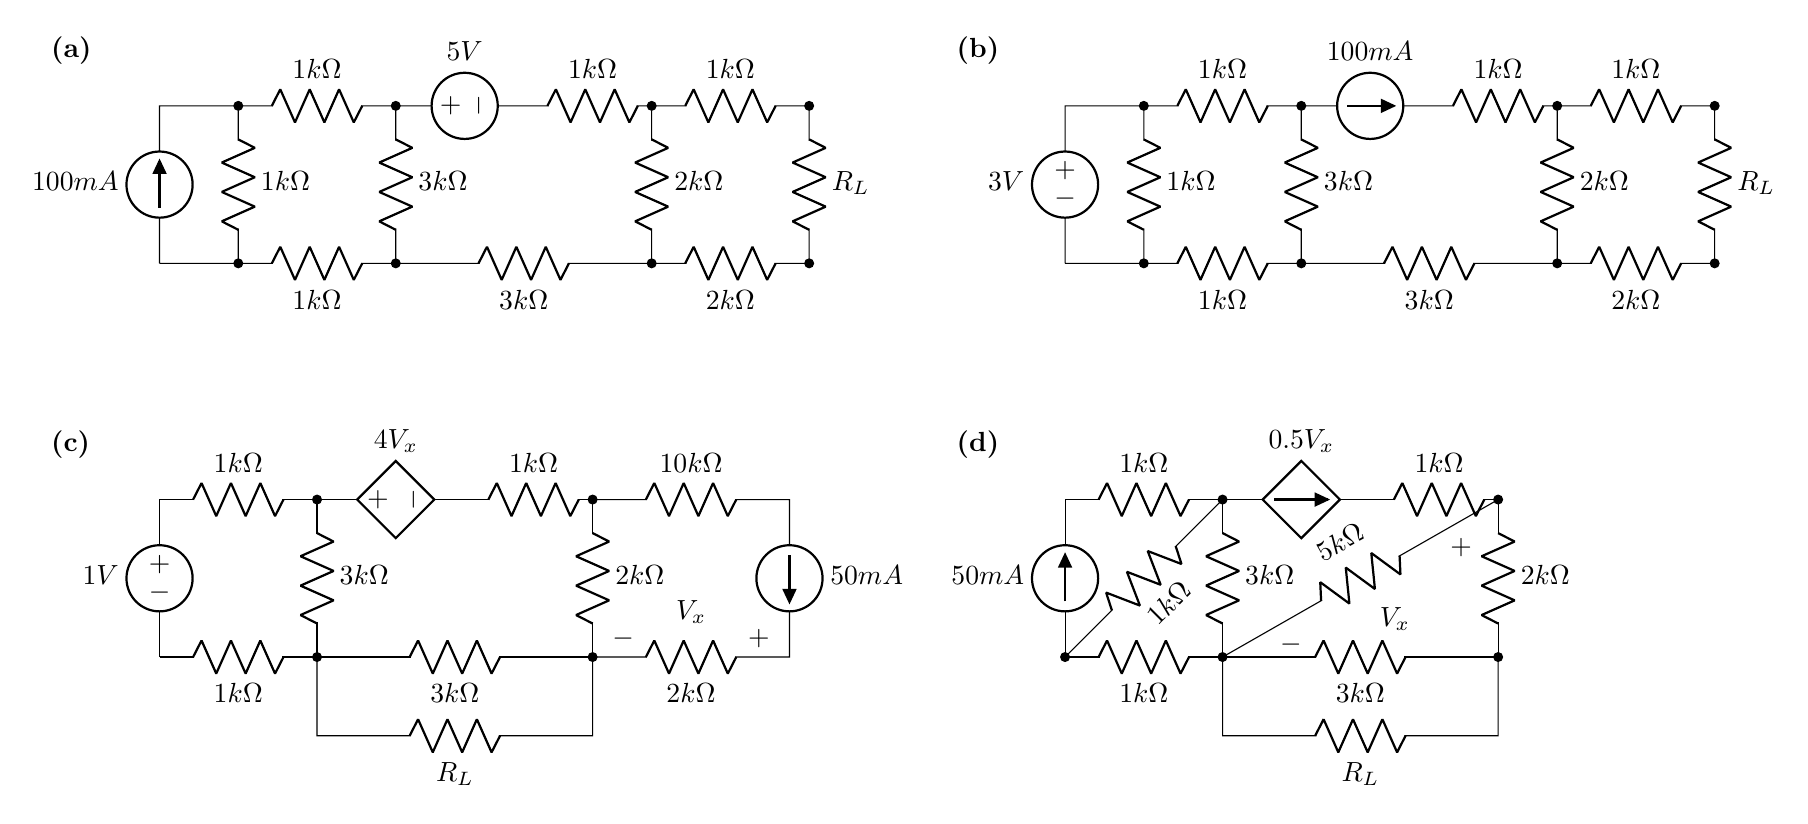
\begin{tikzpicture}

% (a)
\begin{scope}
    % Display the tile.
    \node[anchor=north west, color=black] at (-3.5, 3) {\textbf{(a)}};
    % Defining nodes.
    \draw (-1.0, 2) node[circ] (O1) {};
    \draw (-1.0, 0) node[circ] (O2) {};
    \draw (1, 2) node[circ] (A1) {};
    \draw (1, 0) node[circ] (A2) {};
    \draw (4.25, 2) node[circ] (B1) {};
    \draw (4.25, 0) node[circ] (B2) {};
    \draw (6.25, 2) node[circ] (C1) {};
    \draw (6.25, 0) node[circ] (C2) {};
    \draw (-2, 0) to[I, l={$100mA$}] ++(0, 2) to (O1) to[R, l=$1k\Omega$] (O2) to (-2, 0); 
    \draw (O1) to[R, l=$1k\Omega$] (A1) to[R, l=$3k\Omega$] (A2) to[R, l=$1k\Omega$] (O2);
    % \draw (O1) to[R, l=$1k\Omega$] (O2);
    \draw (A1) to [V, l=$5V$] ++(1.75, 0) to[R, l=$1k\Omega$] (B1) to[R, l=$2k\Omega$] (B2) to[R, l=$3k\Omega$] (A2);
    \draw (B1) to [R, l=$1k\Omega$] (C1) to[R, l=$R_L$] (C2) to[R, l=$2k\Omega$] (B2);
\end{scope}

% (b)
\begin{scope}[xshift=11.5cm]
    % Display the tile.
    \node[anchor=north west, color=black] at (-3.5, 3) {\textbf{(b)}};
    % Defining nodes.
    \draw (-1.0, 2) node[circ] (O1) {};
    \draw (-1.0, 0) node[circ] (O2) {};
    \draw (1, 2) node[circ] (A1) {};
    \draw (1, 0) node[circ] (A2) {};
    \draw (4.25, 2) node[circ] (B1) {};
    \draw (4.25, 0) node[circ] (B2) {};
    \draw (6.25, 2) node[circ] (C1) {};
    \draw (6.25, 0) node[circ] (C2) {};
    \draw (-2, 0) to[V, l={$3V$}, invert] ++(0, 2) to (O1) to[R, l=$1k\Omega$] (O2) to (-2, 0);
    \draw (O1) to[R, l=$1k\Omega$] (A1) to[R, l=$3k\Omega$] (A2) to[R, l=$1k\Omega$] (O2);
    \draw (A1) to [I, l=$100mA$] ++(1.75, 0) to[R, l=$1k\Omega$] (B1) to[R, l=$2k\Omega$] (B2) to[R, l=$3k\Omega$] (A2);
    \draw (B1) to [R, l=$1k\Omega$] (C1) to[R, l=$R_L$] (C2) to[R, l=$2k\Omega$] (B2);
\end{scope}

% (c)
\begin{scope}[yshift=-5cm]
    % Display the tile.
    \node[anchor=north west, color=black] at (-3.5, 3) {\textbf{(c)}};
    % Defining nodes.
    \draw (0, 2) node[circ] (A1) {};
    \draw (0, 0) node[circ] (A2) {};
    \draw (3.5, 2) node[circ] (B1) {};
    \draw (3.5, 0) node[circ] (B2) {};
    \draw (-2, 0) to[V, l={$1V$}, invert] ++(0, 2) to[R, l=$1k\Omega$] (A1) to[R, l=$3k\Omega$] (A2) to[R, l=$1k\Omega$] (-2, 0);
    \draw (A1) to[cV, l^=$4V_x$] ++(2, 0) to[R, l=$1k\Omega$] (B1) to[R, l=$2k\Omega$] (B2) to[R, l=$3k\Omega$] (A2);
    \draw (B1) to [R, l=$10k\Omega$] ++(2.5, 0) to[I, l=$50mA$] ++(0, -2) to[R, l=$2k\Omega$, v_>=$V_x$] (B2);
    \draw (A2) to ++(0, -1) to[R, l_=$R_L$] ++(3.5, 0) to (B2);
\end{scope}

% (d)
\begin{scope}[xshift=11.5cm, yshift=-5cm]
    % Display the tile.
    \node[anchor=north west, color=black] at (-3.5, 3) {\textbf{(d)}};
    % Defining nodes.
    \draw (-2, 0) node[circ] (O2) {};
    \draw (0, 2) node[circ] (A1) {};
    \draw (0, 0) node[circ] (A2) {};
    \draw (3.5, 2) node[circ] (B1) {};
    \draw (3.5, 0) node[circ] (B2) {};
    \draw (-2, 0) to[I, l={$50mA$}] ++(0, 2) to[R, l=$1k\Omega$] (A1) to[R, l=$3k\Omega$] (A2) to[R, l=$1k\Omega$] (-2, 0);
    \draw (A1) to[R, l=$1k\Omega$] (O2);
    \draw (A1) to[cI, l^=$0.5 V_x$] ++(2, 0) to[R, l=$1k\Omega$] (B1) to[R, l=$2k\Omega$] (B2) to[R, l=$3k\Omega$] (A2);
    \draw (B1) to[R, l_=$5k\Omega$, v^>=$V_x$] (A2);
    \draw (A2) to ++(0, -1) to[R, l_=$R_L$] ++(3.5, 0) to (B2);
    % \draw (B1) to [R, l=$10k\Omega$] ++(2.5, 0) to[I, l=$50mA$] ++(0, -2) to[R, l=$2k\Omega$, v_>=$V_x$] (B2);
    % \draw (A2) to ++(0, -1) to[R, l_=$R_L$] ++(3.5, 0) to (B2);
\end{scope}

% % Plot 2: Step Function
% \begin{scope}[xshift=9cm]
%     % Display the tile.
%     \node[anchor=north west, color=black] at (0, 3) {\textbf{(b)} Step Function};
%     \begin{axis}[
%         name=plot2,
%         % at={(plot1.right of south east)}, anchor=left of south west,
%         width=8cm,
%         height=4cm,
%         xlabel={$t$},
%         ylabel={$v(t)$},
%         xmin=0, xmax=5,
%         ymin=-0.25, ymax=1.25,
%         axis lines=left,
%         axis line style={->},
%         legend style={
%             at={(1.05,1.0)},
%             anchor=north west,
%             draw=none,
%             align=left
%         },
%         thick,
%         samples=1000,
%         domain=0:5,
%         grid=major,
%         major grid style={dotted, black}
%     ]
%     \addplot[myred, ultra thick] coordinates {
%         (0, 0)
%         (1, 0)
%         (1, 1)
%         (5, 1)
%     };
%     \end{axis}
% \end{scope}


% % Plot 3: Arbitrary Function
% \begin{scope}[yshift=-4cm]
%     % Display the tile.
%     \node[anchor=north west, color=black] at (0, 3) {\textbf{(c)} Arbitrary Function};
%     \begin{axis}[
%         name=plot2,
%         % at={(plot1.right of south east)}, anchor=left of south west,
%         width=8cm,
%         height=4cm,
%         xlabel={$t$},
%         ylabel={$v(t)$},
%         xmin=0, xmax=10,
%         ymin=-1, ymax=5,
%         axis lines=left,
%         axis line style={->},
%         legend style={
%             at={(1.05,1.0)},
%             anchor=north west,
%             draw=none,
%             align=left
%         },
%         thick,
%         samples=1000,
%         domain=0:5,
%         grid=major,
%         major grid style={dotted, black}
%     ]
%     \addplot[myred, ultra thick] coordinates {
%         (0, 0)
%         (1, 2)
%         (3, 2)
%         (4, 4)
%         (5, 0)
%         (6, 4)
%         (8, 4)
%         (9, 1)
%         (10, 0)
%     };
%     \end{axis}
% \end{scope}

\end{tikzpicture}

\end{document}